\documentclass{article}

\usepackage{graphicx}
\usepackage[final]{nips_2017}


\usepackage{polski}
\usepackage[utf8]{inputenc} % allow utf-8 input
\usepackage[T1]{fontenc}    % use 8-bit T1 fonts
\usepackage{hyperref}       % hyperlinks
\usepackage{url}            % simple URL typesetting
\usepackage{booktabs}       % professional-quality tables
\usepackage{amsfonts}       % blackboard math symbols
\usepackage{nicefrac}       % compact symbols for 1/2, etc.
\usepackage{microtype}      % microtypography

\title{ Sprawozdanie 1 }


\author{
  Konrad Gmyrek\\
  247008
}

\begin{document}
% \nipsfinalcopy is no longer used

\maketitle

\begin{abstract}
  Poniżej przeprowadzono kilka badań dla Perceptronu prostego oraz Adaline, w których badany jest wpływ różnych hiperparametrów na szybkość uczenia. Głównym celem tych badań było sprawdzenie jak poszczególne hiperparametry wpływają na modele oraz wyrobienie sobie intuicji odnośnie działania Perceptronu oraz Adaline.\\Repozyturium kodu: \url{https://github.com/KonradGmy/Lab01}
\end{abstract}

\newpage
\section{Badania Perceptronu}

Poniżej zostały przedstawione wyniki badań dla Perceptronu. Perceptron symuluje działanie funkcji AND dla dwóch zmiennych w logice bipolarnej. Perceptron przestaje aktualizować wagi gdy w epoce nie pojawi się błąd. Każde badanie dla klarowności zostało przeprowadzone sto razy (wyniki dla dziesięciu powtórzeń często znacząco się różniły dlatego też zwiększyłem liczbe powtórzeń danego badania)

\subsection{Badanie 1}

Zbadany został wpływ progu $\theta$ na szybkość uczenia Perceptronu prostego, wagi początkowe wektora W zostały wybrane z przedziału (-0,01, 0,01), wartość współczynnika uczenia $\alpha$ wynosi 0,1. Dla każdej wartości progu $\theta$ badanie zostało powtórzone sto razy, poniżej uśrednione wyniki badania.\\


\begin{table}[h]
  \centering
  \caption{Wpływ $\theta$ na szybkość uczenia}
  \begin{tabular}{lllllll}
    \toprule
    $\theta$ & 0.01 & 0.1 & 0.5 & 1 & 2 & 5 \\
    epoki & 2.0 & 2.0 & 2.0 & 3.8 & 5.8 & 11.77 \\
    \bottomrule
  \end{tabular}
\end{table}


\begin{center}
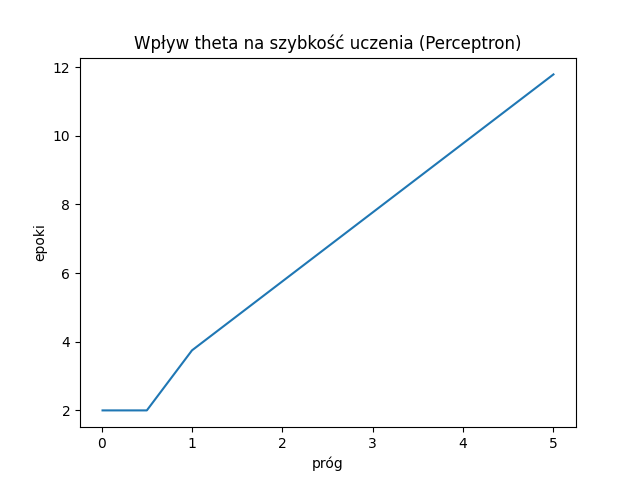
\includegraphics[scale=0.8]{per_exp1.png}
\end{center}

Wnioski: Zależność szybkości uczenia oraz progu $\theta$ jest widocznie liniowa, im większy próg tym średnio więcej epok potrzeba do wyuczenia neuronu. Dzieje się tak dlatego, że dla małych wag wektora W oraz dużego progu potrzeba więcej epok na znalezienie odpowiedniej prostej która będzie klasyfikować dane.

\newpage
\subsection{Badanie 2}

Zbadany został wpływ zakresu w jakim losowane są początkowe wagi wektora W na szybkość uczenia. Waga początkowa progu $\theta$ została wylosowana z przedziału (-1, 1), wartość współczynnika uczenia $\alpha$ wynosi 0,1. Dla każdej wartości zakresu badanie zostało powtórzone sto razy, poniżej uśrednione wyniki badania.\\


\begin{table}[h]
  \centering
  \caption{Wpływ zakresu wag W na szybkość uczenia}
  \begin{tabular}{lllllll}
    \toprule
    zakres & (-1, 1) & (-0.8, 0.8) & (-0.5, 0.5) & (-0.2, 0.2) & (-0.05, 0.05) \\
    epoki & 3.36 & 3.14 & 2.97 & 2.9 & 2.68 \\
    \bottomrule
  \end{tabular}
\end{table}


\begin{center}
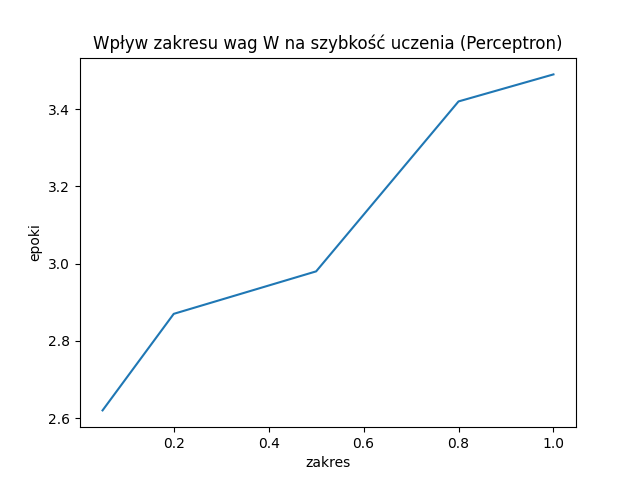
\includegraphics[scale=0.8]{per_exp2.png}
\end{center}

Wnioski: Zależnośc szybkości uczenia i zakresu początkowego wektora W jest ponownie liniowa, im bardziej losowe wartości wag tym średnio więcej epok potrzebnych do wyuczenia neuronu. Gdy współczynnik uczenia $\alpha$ jest mały, wartości wektora W zmieniają się powoli, a zatem potrzeba więcej epok zanim znajdziemy odpowiedni wektor W. \\

\newpage
\subsection{Badanie 3}

Zbadany został wpływ współczynnika uczenia $\alpha$ na szybkość uczenia. Waga początkowa progu $\theta$ została wylosowana z przedziału (-1, 1), wagi początkowe wektora W zostały wybrane z przedziału (-0,01, 0,01). Dla każdej wartości wspołczynnika uczenia badanie zostało powtórzone sto razy, poniżej uśrednione wyniki badania.\\


\begin{table}[h]
  \centering
  \caption{Wpływ współczynnika uczenia na szybkość uczenia}
  \begin{tabular}{llllllllll}
    \toprule
    $\alpha$ & 0.01 & 0.1 & 0.2 & 0.3 & 0.4 & 0.5 & 1 & 2 & 5 \\
    epoki & 10.01 & 2.51 & 2.21 & 2.34 & 2.36 & 2.49 & 2.56 & 2.42 & 2.56 \\
    \bottomrule
  \end{tabular}
\end{table}


\begin{center}
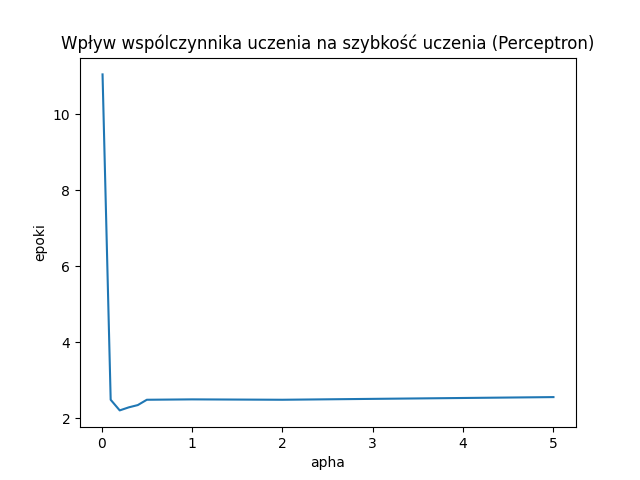
\includegraphics[scale=0.8]{per_exp3.png}
\end{center}

Wnioski: Dla niskich wartości $\alpha$ liczba epok potrzebnych do wyuczenia neuronu jest bardzo duża ponieważ potrzeba więcej czasu na znalezienie odpowiednich wartości wektora W, dalej z kolei dla wartości większych niż 1 liczba epok utrzymuje się mniej więcej poniżej trzech. Optymalna wartość $\alpha$ dla tego zadania wynosi około 0,2.\\
\newpage
\subsection{Badanie 4}

Zbadany został wpływ logiki na szybkość uczenia. Waga początkowa progu $\theta$ została wylosowana z przedziału (-1, 1), wagi początkowe wektora W zostały wybrane z przedziału (-0,01, 0,01), wartość współczynnika uczenia $\alpha$ wynosi 0,1. Dla każdej logiki badanie zostało powtórzone sto razy, poniżej uśrednione wyniki badania.\\


\begin{table}[h]
  \centering
  \caption{Wspływ logiki na szybkość uczenia}
  \begin{tabular}{lll}
    \toprule
    & logika unipolarna & logika biloparna \\
    epoki & 6.65 & 2.54 \\
    \bottomrule
  \end{tabular}
\end{table}


\begin{center}
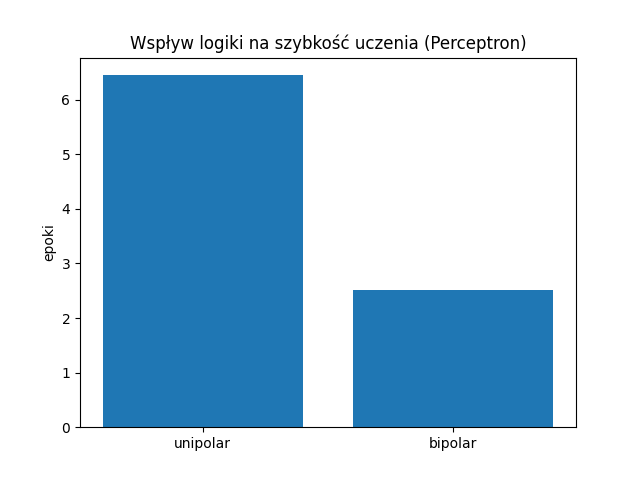
\includegraphics[scale=0.8]{per_exp4.png}
\end{center}

Wnioski: Perceptron prosty dla logiki unipolarnej uczy się zdecydowanie wolniej niż dla logiki bipolarnej. Dzieje się tak dlatego, że w logice bipolarnej przestrzeń w której rozwiązanie jest poprawne jest większa oraz błędy mogą wynosić -2, 0 oraz 2, dlatego też w tym przypadku szybciej jest trafić na odpowiednie rozwiązanie.\\

\newpage
\section{Badania Adaline}

Poniżej zostaną przedstawione wyniki badań dla Adaline. Adaline symuluje działanie funkcji AND and dwóch zmiennych w logice bipolarnej. Każde badanie również zostało przeprowadzone sto razy. Adaline przestaje aktualizować wagi gdy wartość błędu średniokwadratowego spadnie poniżej progu błędu.

\subsection{Badanie 5}

Zbadany został wpływ zakresu w jakim losowane są początkowe wagi wektora W na szybkość uczenia. Waga początkowa progu $\theta$ została wylosowana z przedziału (-1, 1), wartość współczynnika uczenia $\alpha$ wynosi 0,1, wartość progu błędu wynosi 0,4. Dla każdej wartości zakresu badanie zostało powtórzone sto razy, poniżej uśrednione wyniki badania.\\


\begin{table}[h]
  \centering
  \caption{Wpływ zakresu wag na szybkość uczenia}
  \begin{tabular}{llllll}
    \toprule
    zakres & (-1, 1) & (-0.8, 0.8) & (-0.5, 0.5) & (-0.2, 0.2) & (-0.05, 0.05) \\
    epoki & 4.45 & 4.35 & 4.17 & 3.96 & 3.99 \\
    \bottomrule
  \end{tabular}
\end{table}


\begin{center}
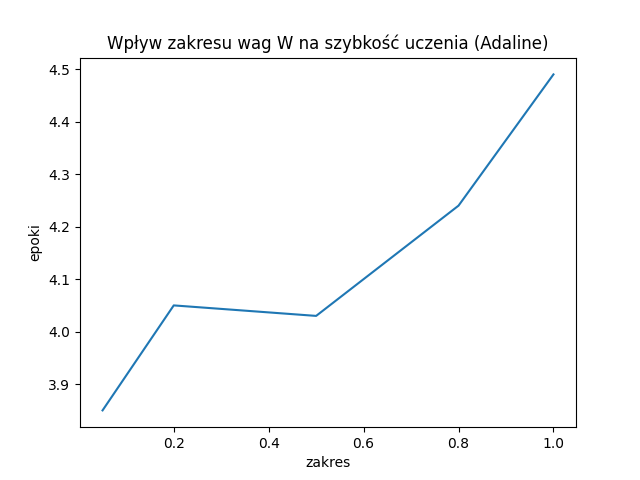
\includegraphics[scale=0.8]{ada_exp1.png}
\end{center}

Wnioski: Zależnośc szybkości uczenia i zakresu początkowego wektora W dla Adaline jest tak samo jak w przypadku Perceptronu liniowa, im bardziej losowe wartości wag tym średnio więcej epok potrzebnych do wyuczenia neuronu, powód takiej zależności również jest taki sam jak w przypadku Perceptronu.

\newpage
\subsection{Badanie 6}

Zbadany został wpływ współczynnika uczenia $\alpha$ na szybkość uczenia. Waga początkowa progu $\theta$ została wylosowana z przedziału (-1, 1), wagi początkowe wektora W zostały wybrane z przedziału (-0,01, 0,01), wartość progu błędu wynosi 0,4. Dla każdej wartości współczynnika uczenia $\alpha$ badanie zostało powtórzone sto razy, poniżej uśrednione wyniki badania.\\


\begin{table}[h]
  \centering
  \caption{Wpływ wspólczynnika uczenia na szybkość uczenia}
  \begin{tabular}{llllll}
    \toprule
    $\alpha$ & 0.001 & 0.01 & 0.1 & 1 \\
    epoki & 100.0 & 24.94 & 3.98 & 67.33 \\
    \bottomrule
  \end{tabular}
\end{table}


\begin{center}
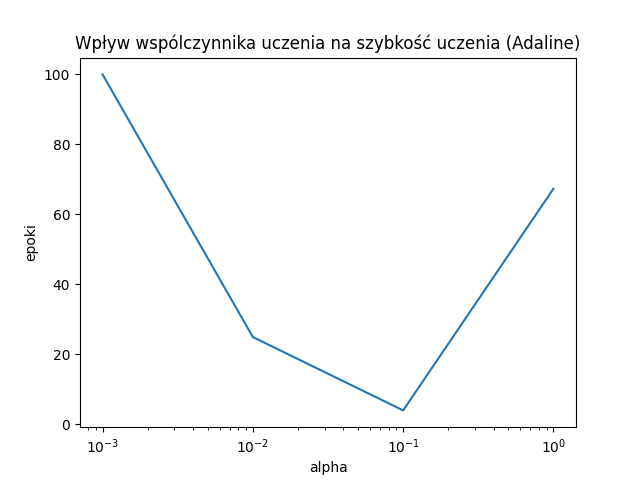
\includegraphics[scale=0.8]{ada_exp2.png}
\end{center}

Wnioski: Adaline reaguje o wiele gorzej na zmiany współczynnika uczenia, dla bardzo małych wartości $\alpha$ neuron nie był w stanie wyuczyć się w mniej niż 100 epokach, najlepsza wartość $\alpha$ wynosła dla tego zadania 0,1. Dla wartości $\alpha$ większych niż 1 nie jesteśmy w stanie znaleźć rozwiązania ponieważ błędy zamiast maleć, rosną w nieskończoność.

\newpage
\subsection{Badanie 7}

Zbadany został wpływ wartości progu błędu na szybkość uczenia. Waga początkowa progu $\theta$ została wylosowana z przedziału (-1, 1), wagi początkowe wektora W zostały wybrane z przedziału (-0,01, 0,01), wagi początkowe wektora W zostały wybrane z przedziału (-0,01, 0,01). Dla każdej wartości progu błędu badanie zostało powtórzone sto razy, poniżej uśrednione wyniki badania.\\


\begin{table}[h]
  \centering
  \caption{Wpływ progu błędu na szybkość uczenia}
  \begin{tabular}{llllllllll}
    \toprule
    próg & 0.2 & 0.3 & 0.4 & 0.5 & 0.6 & 0.7 & 0.8 & 0.9 & 1 \\
    epoki & 100.0 & 100.0 & 4.0 & 3.04 & 2.52 & 2.27 & 2.06 & 1.83 & 1.6 \\
    \bottomrule
  \end{tabular}
\end{table}


\begin{center}
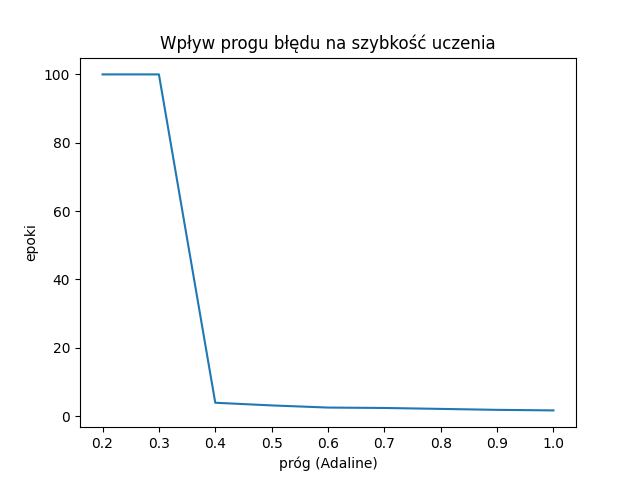
\includegraphics[scale=0.8]{ada_exp3.png}
\end{center}

Wnioski: Dla niskich wartości progu błędu (poniżej 0,4) neuron nie jest w stanie osiągnać błędu mniejszego niż próg w mniej niż 100 epokach. Dla wartości większych niż obserwujemy zależność liniową jednak nie znaczy to że wyższy próg jest lepszy ponieważ dla wartości progu blędu równego neuron kończy proces uczenia pomimo tego że nie zwraca poprawnych wyników.

\newpage
\section{Porównanie wyników badań dla Perceptronu i Adaline}
Poniżej przedstawione zostały porównania poszczególych badań dla Perceptronu prostego i Adaline.

\subsection{Porównanie wpływu zakresu wag wektora W na szybkość uczenia}

\begin{center}
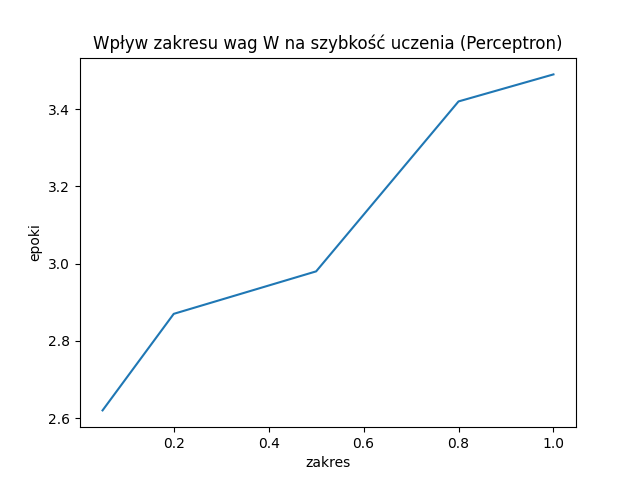
\includegraphics[scale=0.7]{per_exp2.png}
\end{center}
\begin{center}
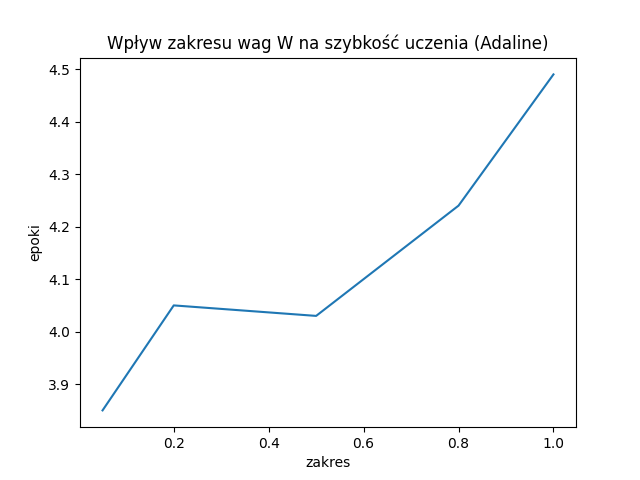
\includegraphics[scale=0.7]{ada_exp1.png}
\end{center}
Wnioski: W dla obu modeli obserwujemy liniową zależność pomiędzy zakresem początkowym losowanych wartości wag wektora W, a ilościa epok potrzebnych do wyuczenia modelu.

\newpage
\subsection{Porównanie wpływu współczynnika uczenia na szybkość uczenia}

\begin{center}
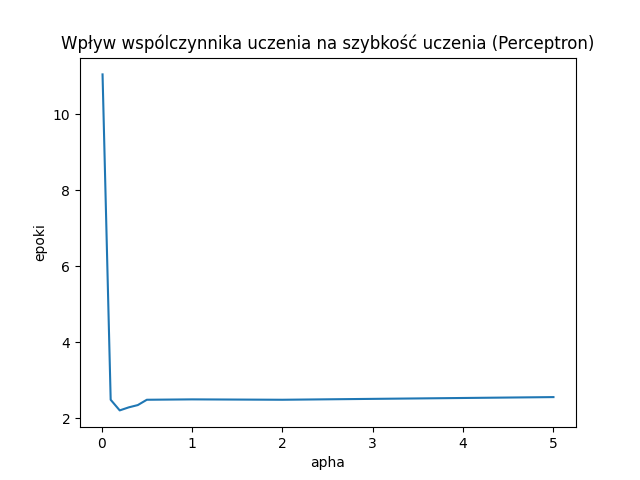
\includegraphics[scale=0.7]{per_exp3.png}
\end{center}
\begin{center}
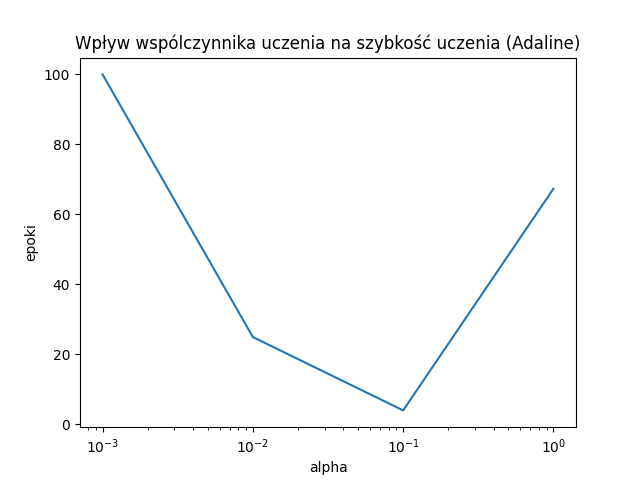
\includegraphics[scale=0.7]{ada_exp2.png}
\end{center}
Wnioski: Na wykresach widoczna jest wyraźna różnica pomiędzy wpływem współczynnika uczenia $\alpha$ na Perceptron oraz na Adaline, w przypadku tego drugiego, zbyt małe lub zbyt duże $\alpha$ powoduje to, że model nie jest w stanie wyuczyć się w mniej niż 100 epok.

\newpage
\subsection{Porównanie Perceptronu i Adaline dla znalezionych hiperparametrów}

Poniżej przedstawione wyniki badania szybkości uczenia Perceptronu i Adaline dla optymalnych hiperparametrów. Dla każdego modelu badanie zostało powtórzone sto razy, poniżej uśrednione wyniki badania.\\

\begin{table}[h]
  \centering
  \caption{Dobrane hiperparametry}
  \begin{tabular}{lllll}
    \toprule
    Perceptron & $\theta$ $\in$ (-0.5, 0.5) & $\alpha$ = 0.2 & $W_i$ $\in$ (-0.1, 0.1) & model = bipolar  \\
    Adaline & $\theta$ $\in$ (-0.5, 0.5) & $\alpha$ = 0.1 & $W_i$ $\in$ (-0.2, 0.2) & threshold = 0.6\\
    \bottomrule
  \end{tabular}
\end{table}

\begin{table}[h]
  \centering
  \caption{Wpływ modelu na szybkość uczenia}
  \begin{tabular}{ll}
    \toprule
    Perceptron & Adaline \\
    2.58 & 2.45 \\
    \bottomrule
  \end{tabular}
\end{table}


\begin{center}
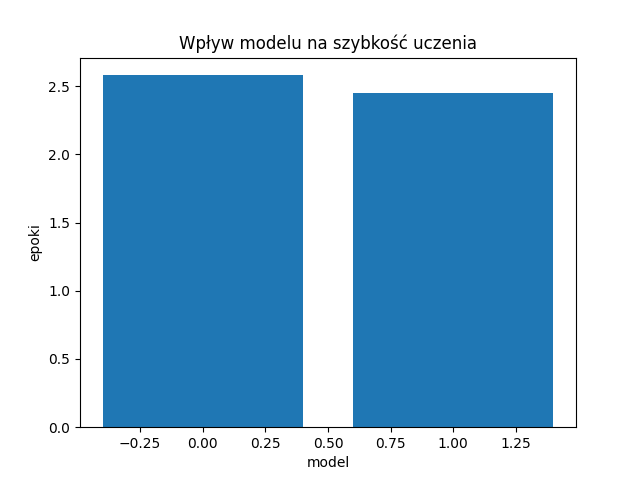
\includegraphics[scale=0.8]{ada_exp4.png}
\end{center}

Wnioski: Dla obydwu modeli średnia liczba epok potrzebnych do wyuczenia modelu jest zbliżona, jednak modele różnią się od siebie w znaczący sposób i mają swoje mocna i słabe strony. Perceptron kończy proces uczenia gdy znajdzie pierwsze poprawne rozwiązanie co może prowadzić do tego, że gdy podstawimy mu dane inne niż testowe będzie je klasyfikował błędnie, Adaline z kolei może nigdy nie znaleźć odpowiednio niskiego błędu, a dla złego $\alpha$ może nigdy się nie wyuczyć, za to nie jest mniejsze prawdopodobnieństwo problemu zbytniego dopasowania się do danych testowych, ponieważ Adaline znajduje lepszą prostą klasyfikującą dane, nieleżacą w pobliżu żadnej z klas.

\end{document}
